\documentclass[9pt,twocolumn,twoside,]{pnas-new}

%% Some pieces required from the pandoc template
\providecommand{\tightlist}{%
  \setlength{\itemsep}{0pt}\setlength{\parskip}{0pt}}

% Use the lineno option to display guide line numbers if required.
% Note that the use of elements such as single-column equations
% may affect the guide line number alignment.


\usepackage[T1]{fontenc}
\usepackage[utf8]{inputenc}



\templatetype{pnasresearcharticle}  % Choose template

\title{A Standardized Effect Size for Evaluating and Comparing the Strength of
Phylogenetic Signal}

\author[a]{Dean C. Adams}
\author[a,b]{Erica K. Baken}
\author[b]{Michael L. Collyer}

  \affil[a]{Department of Ecology, Evolution, and Organismal Biology, Iowa State
University, Ames, Iowa, USA.}
  \affil[b]{Department of Science, Chatham University, Pittsburgh, Pennsylvania,
USA.}


% Please give the surname of the lead author for the running footer
\leadauthor{Adams et al.}

% Please add here a significance statement to explain the relevance of your work
\significancestatement{Evolutionary biologists wish to quantify and compare the strength of
phylogenetic signal across traits, but analytical tools for these
comparisons are generally lacking. Here we develop a standardized effect
size based on \(\kappa\) (\(Z_\kappa\)), which measures the strength of
phylogenetic signal on a common statistical scale, and provides a
mechanism for formally comparing the strength of phylogenetic signal
across datasets. Additionally, we find that a commonly used parameter
(Pagel's \(\lambda\)) is insuitable for this purpose. Our procedure
enables biologists to quantitatively address hypotheses that compare the
strength of phylogenetic signal between various phenotypic traits, even
when those traits are found in different evolutionary lineages or have
different units or scales.}


\authorcontributions{D.C.A. designed the research; D.C.A., E.K.B., and M.L.C. performed the
research and wrote the paper.}

\authordeclaration{The authors declare no conflict of interest.}


\correspondingauthor{\textsuperscript{} }

% Keywords are not mandatory, but authors are strongly encouraged to provide them. If provided, please include two to five keywords, separated by the pipe symbol, e.g:
 \keywords{  phylogenetic signal |  macroevolution |  lambda |  kappa  } 

\begin{abstract}
Macroevolutionary studies frequently characterize the phylogenetic
signal in phenotypes, and wish to compare the strength of that signal
across traits. However, analytical tools for such comparisons have
largely remained underdeveloped. Here we evaluate the efficacy of one
commonly used parameter (Pagel's \(\lambda\)) to estimate the strength
of phylogenetic signal in phenotypic traits, and evaluate the degree to
which \(\lambda\) correctly identifies known levels of phylogenetic
signal. We find that \(\lambda\) behaves as a Bernoulli random variable,
and that estimates are increasingly skewed at larger and smaller input
levels of phylogenetic signal. Further, the precision of \(\lambda\) in
estimating actual levels of phylogenetic signal is often inaccurate, and
biological interpretations of the strength of phylogenetic signal based
on \(\lambda\) are therefore compromised. We propose a standardized
effect size based on \(\kappa\), (\(Z_\kappa\)), which measures the
strength of phylogenetic signal more reliably than does \(\lambda\), and
places that signal on a common scale for statistical comparison. We
develop tests based on \(Z_\kappa\) to provide a mechanism for formally
comparing the strength of phylogenetic signal across datasets, in much
the same manner as effect sizes may be used to summarize patterns in
quantitative meta-analysis. Our approach extends the phylogenetic
comparative toolkit to address hypotheses that compare the strength of
phylogenetic signal between various phenotypic traits, even when those
traits are found in different evolutionary lineages or have different
units or scales.
\end{abstract}

\dates{This manuscript was compiled on \today}
\doi{\url{www.pnas.org/cgi/doi/10.1073/pnas.XXXXXXXXXX}}

\begin{document}

% Optional adjustment to line up main text (after abstract) of first page with line numbers, when using both lineno and twocolumn options.
% You should only change this length when you've finalised the article contents.
\verticaladjustment{-2pt}

\maketitle
\thispagestyle{firststyle}
\ifthenelse{\boolean{shortarticle}}{\ifthenelse{\boolean{singlecolumn}}{\abscontentformatted}{\abscontent}}{}

% If your first paragraph (i.e. with the \dropcap) contains a list environment (quote, quotation, theorem, definition, enumerate, itemize...), the line after the list may have some extra indentation. If this is the case, add \parshape=0 to the end of the list environment.

\acknow{We thank E. Glynne and B. Juarez for comments on early drafts of the
manuscript. This work was supported in part by NSF grant DBI-1902511 (to
D.C.A.) and DBI-1902694 (to M.L.C.).}

This PNAS journal template is provided to help you write your work in
the correct journal format. Instructions for use are provided below.

Note: please start your introduction without including the word
``Introduction'' as a section heading (except for math articles in the
Physical Sciences section); this heading is implied in the first
paragraphs.

\hypertarget{guide-to-using-this-template}{%
\section*{Guide to using this
template}\label{guide-to-using-this-template}}
\addcontentsline{toc}{section}{Guide to using this template}

Please note that whilst this template provides a preview of the typeset
manuscript for submission, to help in this preparation, it will not
necessarily be the final publication layout. For more detailed
information please see the
\href{http://www.pnas.org/site/authors/format.xhtml}{PNAS Information
for Authors}.

\hypertarget{author-affiliations}{%
\subsection*{Author Affiliations}\label{author-affiliations}}
\addcontentsline{toc}{subsection}{Author Affiliations}

Include department, institution, and complete address, with the
ZIP/postal code, for each author. Use lower case letters to match
authors with institutions, as shown in the example. Authors with an
ORCID ID may supply this information at submission.

\hypertarget{submitting-manuscripts}{%
\subsection*{Submitting Manuscripts}\label{submitting-manuscripts}}
\addcontentsline{toc}{subsection}{Submitting Manuscripts}

All authors must submit their articles at
\href{http://www.pnascentral.org/cgi-bin/main.plex}{PNAScentral}. If you
are using Overleaf to write your article, you can use the ``Submit to
PNAS'' option in the top bar of the editor window.

\hypertarget{format}{%
\subsection*{Format}\label{format}}
\addcontentsline{toc}{subsection}{Format}

Many authors find it useful to organize their manuscripts with the
following order of sections; Title, Author Affiliation, Keywords,
Abstract, Significance Statement, Results, Discussion, Materials and
methods, Acknowledgments, and References. Other orders and headings are
permitted.

\hypertarget{manuscript-length}{%
\subsection*{Manuscript Length}\label{manuscript-length}}
\addcontentsline{toc}{subsection}{Manuscript Length}

PNAS generally uses a two-column format averaging 67 characters,
including spaces, per line. The maximum length of a Direct Submission
research article is six pages and a PNAS PLUS research article is ten
pages including all text, spaces, and the number of characters displaced
by figures, tables, and equations. When submitting tables, figures,
and/or equations in addition to text, keep the text for your manuscript
under 39,000 characters (including spaces) for Direct Submissions and
72,000 characters (including spaces) for PNAS PLUS.

\hypertarget{references}{%
\subsection*{References}\label{references}}
\addcontentsline{toc}{subsection}{References}

References should be cited in numerical order as they appear in text;
this will be done automatically via bibtex, e.g.~All references,
including for the SI, should be included in the main manuscript file.
References appearing in both sections should not be duplicated. SI
references included in tables should be included with the main reference
section.

\hypertarget{data-archival}{%
\subsection*{Data Archival}\label{data-archival}}
\addcontentsline{toc}{subsection}{Data Archival}

PNAS must be able to archive the data essential to a published article.
Where such archiving is not possible, deposition of data in public
databases, such as GenBank, ArrayExpress, Protein Data Bank, Unidata,
and others outlined in the Information for Authors, is acceptable.

\hypertarget{language-editing-services}{%
\subsection*{Language-Editing
Services}\label{language-editing-services}}
\addcontentsline{toc}{subsection}{Language-Editing Services}

Prior to submission, authors who believe their manuscripts would benefit
from professional editing are encouraged to use a language-editing
service (see list at www.pnas.org/site/authors/language-editing.xhtml).
PNAS does not take responsibility for or endorse these services, and
their use has no bearing on acceptance of a manuscript for publication.

\begin{figure}
\centering
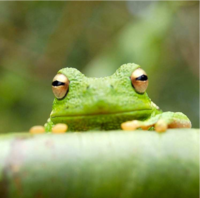
\includegraphics{frog.png}
\caption{Placeholder image of a frog with a long example caption to show
justification setting.{}}
\end{figure}

\hypertarget{sec:figures}{%
\subsection*{Digital Figures}\label{sec:figures}}
\addcontentsline{toc}{subsection}{Digital Figures}

Only TIFF, EPS, and high-resolution PDF for Mac or PC are allowed for
figures that will appear in the main text, and images must be final
size. Authors may submit U3D or PRC files for 3D images; these must be
accompanied by 2D representations in TIFF, EPS, or high-resolution PDF
format. Color images must be in RGB (red, green, blue) mode. Include the
font files for any text.

Figures and Tables should be labelled and referenced in the standard way
using the \texttt{\textbackslash{}label\{\}} and
\texttt{\textbackslash{}ref\{\}} commands.

Figure \[fig:frog\] shows an example of how to insert a column-wide
figure. To insert a figure wider than one column, please use the
\texttt{\textbackslash{}begin\{figure*\}...\textbackslash{}end\{figure*\}}
environment. Figures wider than one column should be sized to 11.4 cm or
17.8 cm wide.

\hypertarget{single-column-equations}{%
\subsection*{Single column equations}\label{single-column-equations}}
\addcontentsline{toc}{subsection}{Single column equations}

Authors may use 1- or 2-column equations in their article, according to
their preference.

To allow an equation to span both columns, options are to use the
\texttt{\textbackslash{}begin\{figure*\}...\textbackslash{}end\{figure*\}}
environment mentioned above for figures, or to use the
\texttt{\textbackslash{}begin\{widetext\}...\textbackslash{}end\{widetext\}}
environment as shown in equation \[eqn:example\] below.

Please note that this option may run into problems with floats and
footnotes, as mentioned in the \href{http://texdoc.net/pkg/cuted}{cuted
package documentation}. In the case of problems with footnotes, it may
be possible to correct the situation using commands
\texttt{\textbackslash{}footnotemark} and
\texttt{\textbackslash{}footnotetext}.

\[\begin{aligned}
(x+y)^3&=(x+y)(x+y)^2\\
       &=(x+y)(x^2+2xy+y^2) \label{eqn:example} \\
       &=x^3+3x^2y+3xy^3+x^3. 
\end{aligned}\]

\hypertarget{supporting-information-si}{%
\subsection*{Supporting Information
(SI)}\label{supporting-information-si}}
\addcontentsline{toc}{subsection}{Supporting Information (SI)}

The main text of the paper must stand on its own without the SI. Refer
to SI in the manuscript at an appropriate point in the text. Number
supporting figures and tables starting with S1, S2, etc. Authors are
limited to no more than 10 SI files, not including movie files. Authors
who place detailed materials and methods in SI must provide sufficient
detail in the main text methods to enable a reader to follow the logic
of the procedures and results and also must reference the online
methods. If a paper is fundamentally a study of a new method or
technique, then the methods must be described completely in the main
text. Because PNAS edits SI and composes it into a single PDF, authors
must provide the following file formats only.

\hypertarget{si-text}{%
\subsubsection*{SI Text}\label{si-text}}
\addcontentsline{toc}{subsubsection}{SI Text}

Supply Word, RTF, or LaTeX files (LaTeX files must be accompanied by a
PDF with the same file name for visual reference).

\hypertarget{si-figures}{%
\subsubsection*{SI Figures}\label{si-figures}}
\addcontentsline{toc}{subsubsection}{SI Figures}

Provide a brief legend for each supporting figure after the supporting
text. Provide figure images in TIFF, EPS, high-resolution PDF, JPEG, or
GIF format; figures may not be embedded in manuscript text. When saving
TIFF files, use only LZW compression; do not use JPEG compression. Do
not save figure numbers, legends, or author names as part of the image.
Composite figures must be pre-assembled.

\hypertarget{d-figures}{%
\subsubsection*{3D Figures}\label{d-figures}}
\addcontentsline{toc}{subsubsection}{3D Figures}

Supply a composable U3D or PRC file so that it may be edited and
composed. Authors may submit a PDF file but please note it will be
published in raw format and will not be edited or composed.

\hypertarget{si-tables}{%
\subsubsection*{SI Tables}\label{si-tables}}
\addcontentsline{toc}{subsubsection}{SI Tables}

Supply Word, RTF, or LaTeX files (LaTeX files must be accompanied by a
PDF with the same file name for visual reference); include only one
table per file. Do not use tabs or spaces to separate columns in Word
tables.

\hypertarget{si-datasets}{%
\subsubsection*{SI Datasets}\label{si-datasets}}
\addcontentsline{toc}{subsubsection}{SI Datasets}

Supply Excel (.xls), RTF, or PDF files. This file type will be published
in raw format and will not be edited or composed.

\hypertarget{si-movies}{%
\subsubsection*{SI Movies}\label{si-movies}}
\addcontentsline{toc}{subsubsection}{SI Movies}

Supply Audio Video Interleave (avi), Quicktime (mov), Windows Media
(wmv), animated GIF (gif), or MPEG files and submit a brief legend for
each movie in a Word or RTF file. All movies should be submitted at the
desired reproduction size and length. Movies should be no more than 10
MB in size.

\hypertarget{still-images}{%
\subsubsection*{Still images}\label{still-images}}
\addcontentsline{toc}{subsubsection}{Still images}

Authors must provide a still image from each video file. Supply TIFF,
EPS, high-resolution PDF, JPEG, or GIF files.

\hypertarget{appendices}{%
\subsubsection*{Appendices}\label{appendices}}
\addcontentsline{toc}{subsubsection}{Appendices}

PNAS prefers that authors submit individual source files to ensure
readability. If this is not possible, supply a single PDF file that
contains all of the SI associated with the paper. This file type will be
published in raw format and will not be edited or composed.

\showmatmethods
\showacknow
\pnasbreak



% Bibliography
% \bibliography{pnas-sample}

\end{document}

